%!TEX ROOT=../../Diplomka.tex

\chapter{Aplikace inverzních úloh}

\section{Porovnání metod inverze SPM12}
V SPM12 toolboxu je naimplementováno 5 algoritmů nedourčených modelů inverzní úlohy (GS, MSP, COH, IID a EBB). Abychom byli schopni metody porovnat, vytvořil jsem několik syntetických datových souborů, které obsahují data, o nichž vím, kde se nachází zdroj jejich aktivity. Syntetická data jsou generována pomocí přímé úlohy, na zvolené souřadnice jsou umístěny proudové dipóly, které generují zvolený průběh proudu. Následně je vypočteno, jak se tyto proudy propagují na skalp modelu a jaké potenciály jsou zaznamenány elektrodami. Funkce pro generování syntetických dat je součástí v SPM12 toolboxu. 

Proces vytváření syntetického datového souboru využívá již existujícího datového souboru s definovanou přímou úlohou, kde jednoduše nahradí označené události nově vypočtenými EEG průběhy se zvolenou úrovní Gaussovského šumu. Datových souborů, ze kterých jsem mohl vycházet, bylo k dispozici několik, vždy jeden od zpracovávaného případu. Náhodně jsem zvolil datový soubor pacienta P110 se 168 označenými událostmi jako výchozí. 

\subsection{Generování syntetických dat}
Vygeneroval jsem celkem 5 scénářů pro porovnání algoritmů inverzních úloh, na nichž jsem následně provedl výpočet inverzní úlohy dostupnými algoritmy:

\begin{itemize}
\item Zdroj v levé hemisféře na pozici [-52, -25, 9] generující průběhy o frekvenci 10 Hz, SNR nastaveno na 0 dB, viz obrázek \ref{scenar1}
\begin{figure}[!h]
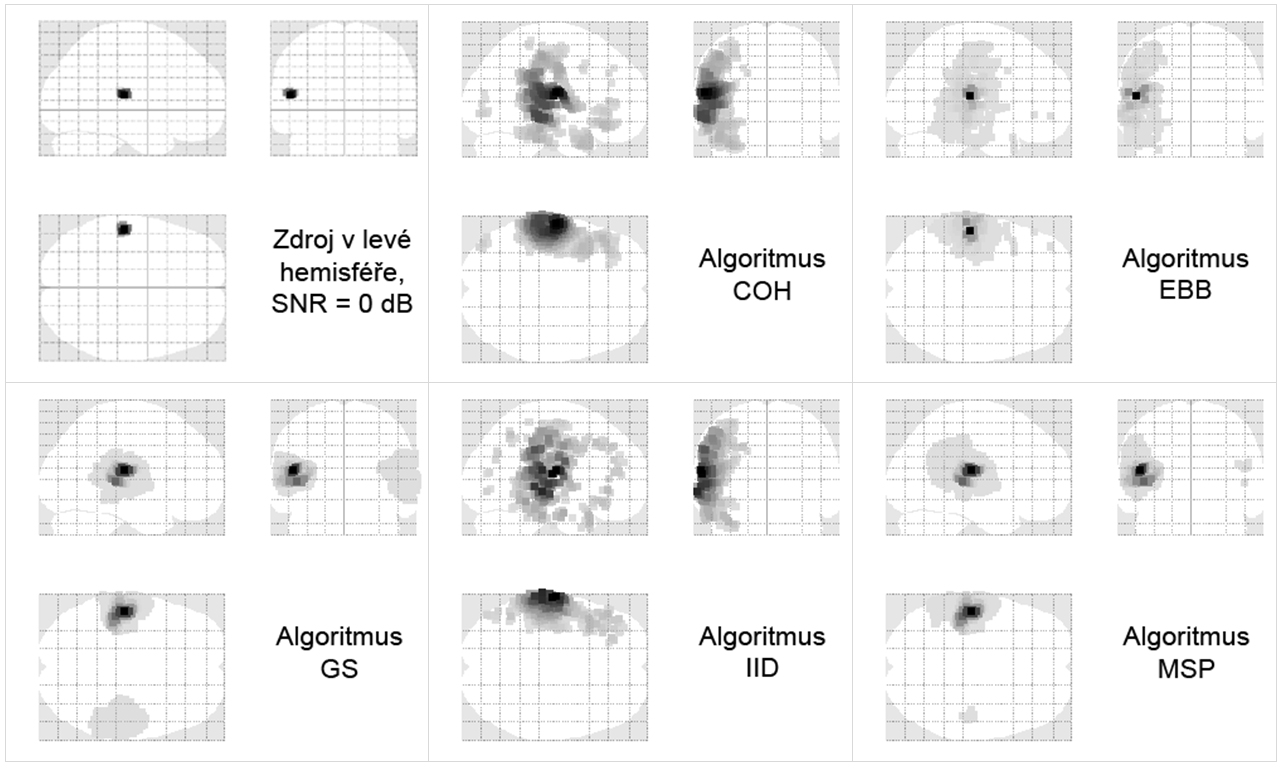
\includegraphics[width=1.0\textwidth]{casti/aplikace/porovnani/scenar1.png}
\caption{Výsledky lokalizace zdroje v levé hemisféře}
\label{scenar1}
\end{figure}

\item Zdroj v pravé hemisféře na pozici [52, -25, 9] generující průběhy o~frekvenci 20 Hz, SNR 0 dB, viz obrázek \ref{scenar2}
\begin{figure}[!h]
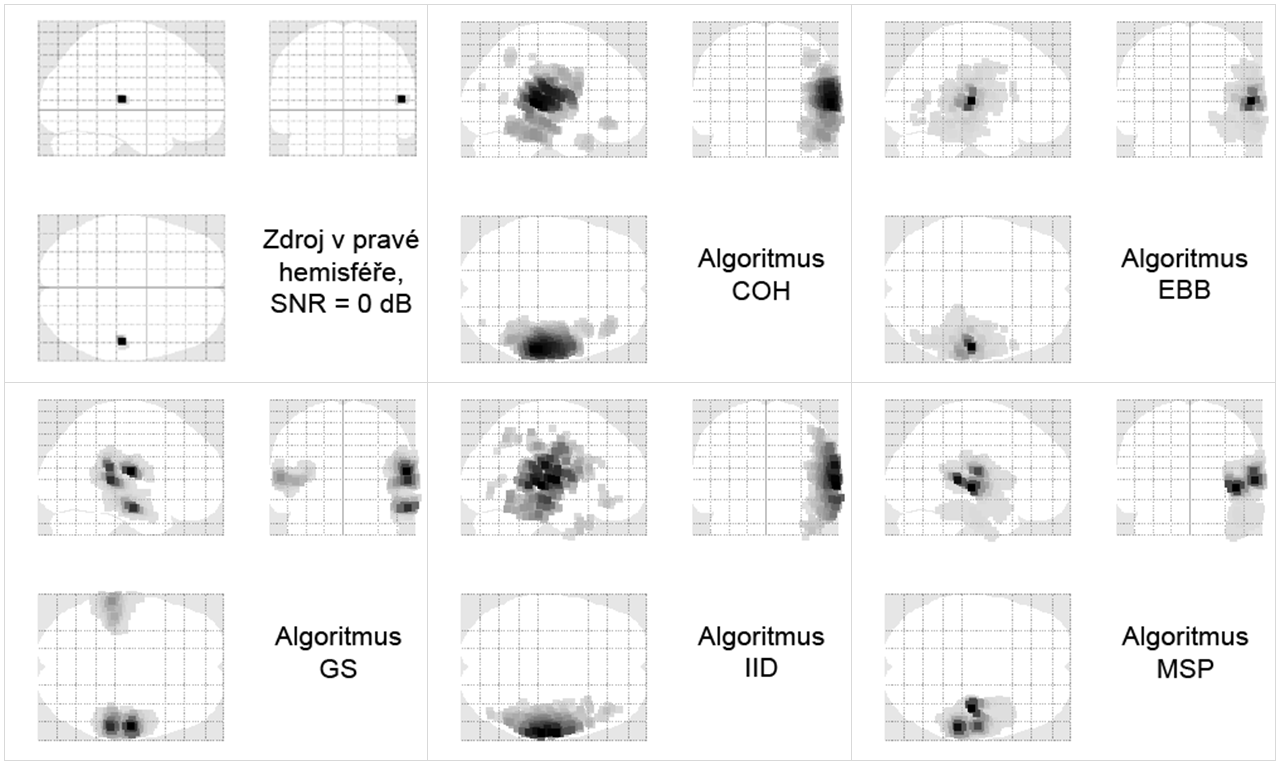
\includegraphics[width=1.0\textwidth]{casti/aplikace/porovnani/scenar2.png}
\caption{Výsledky lokalizace zdroje v pravé hemisféře}
\label{scenar2}
\end{figure}

\item Kombinace předchozích zdrojů v levé a pravé hemisféře, SNR = 10 dB, viz obrázek \ref{scenar3}
\begin{figure}[!h]
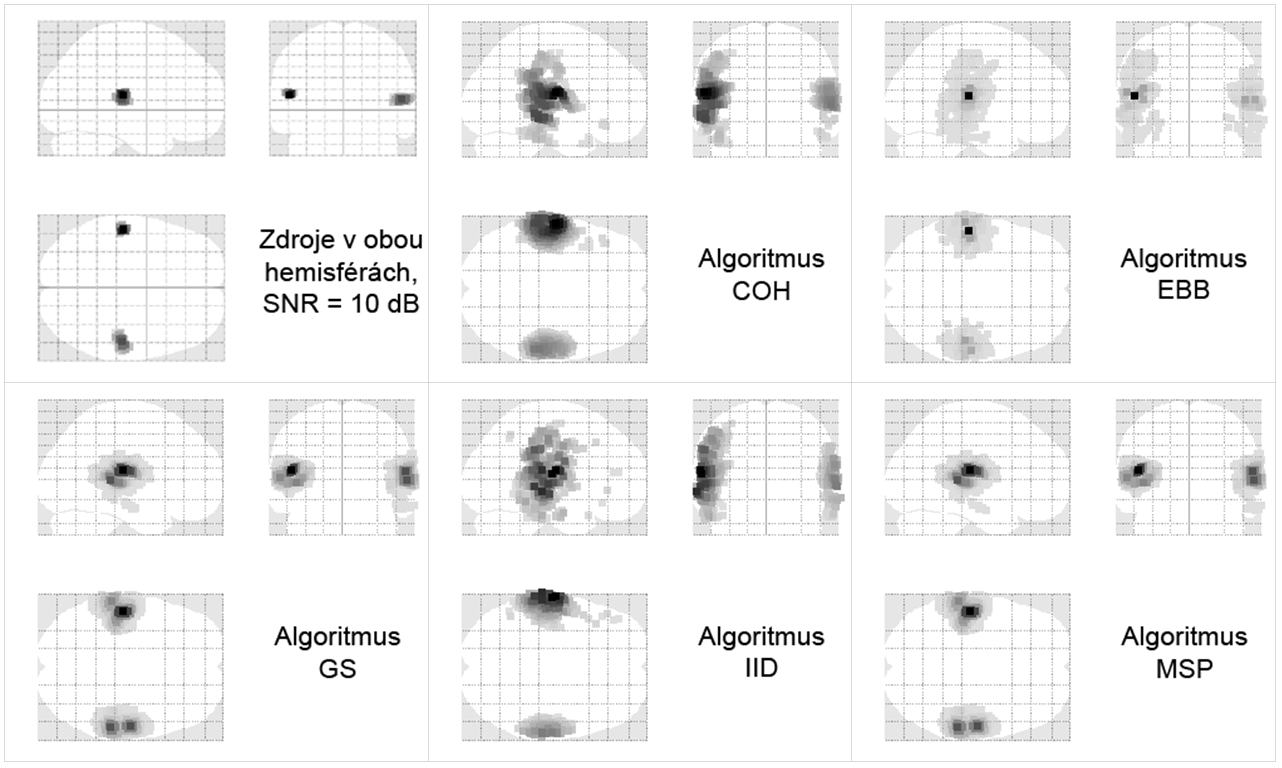
\includegraphics[width=1.0\textwidth]{casti/aplikace/porovnani/scenar3.png}
\caption{Výsledky lokalizace zdroje v pravé i levé hemisféře, při SNR 10 dB}
\label{scenar3}
\end{figure}

\item Kombinace zdrojů s hladinou SNR 0 dB, viz obrázek \ref{scenar4}
\begin{figure}[!h]
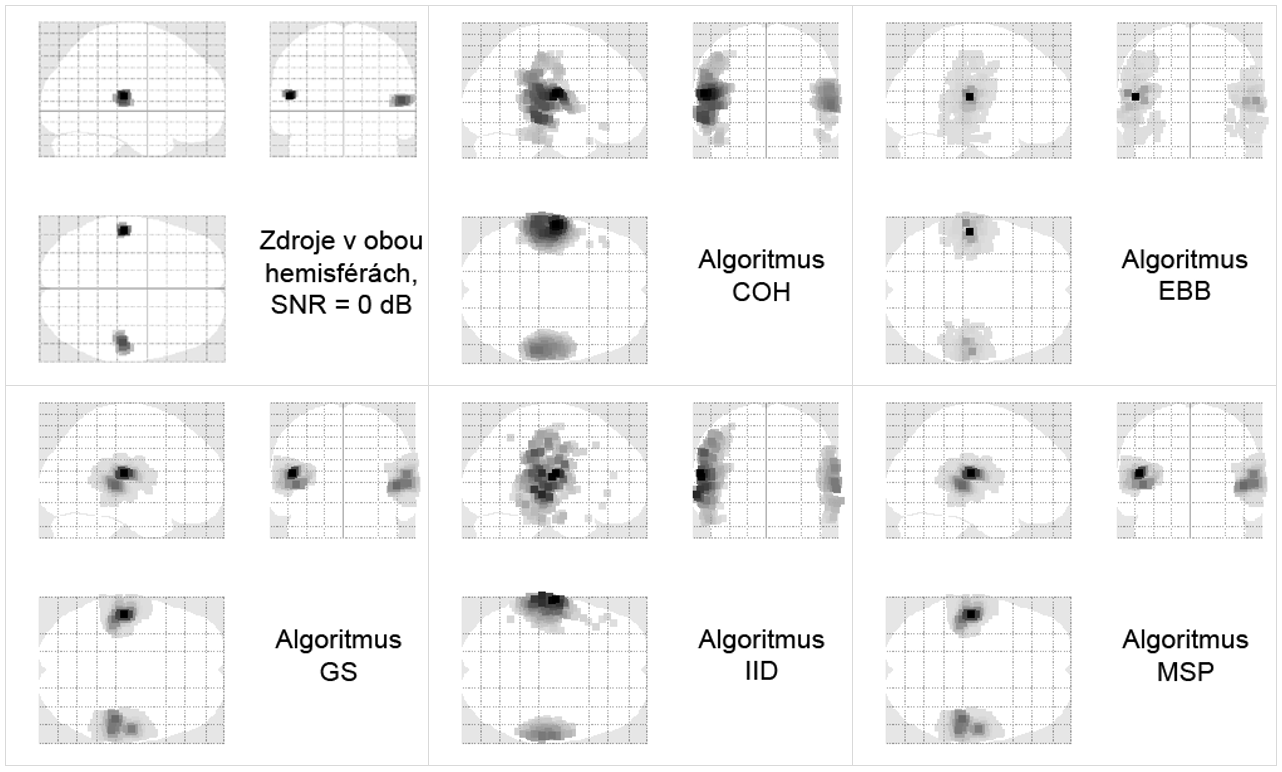
\includegraphics[width=1.0\textwidth]{casti/aplikace/porovnani/scenar4.png}
\caption{Výsledky lokalizace zdroje v pravé i levé hemisféře, při SNR 0 dB}
\label{scenar4}
\end{figure}

\item Kombinace zdrojů s hladinou SNR -10 dB, viz obrázek \ref{scenar5}
\begin{figure}[!h]
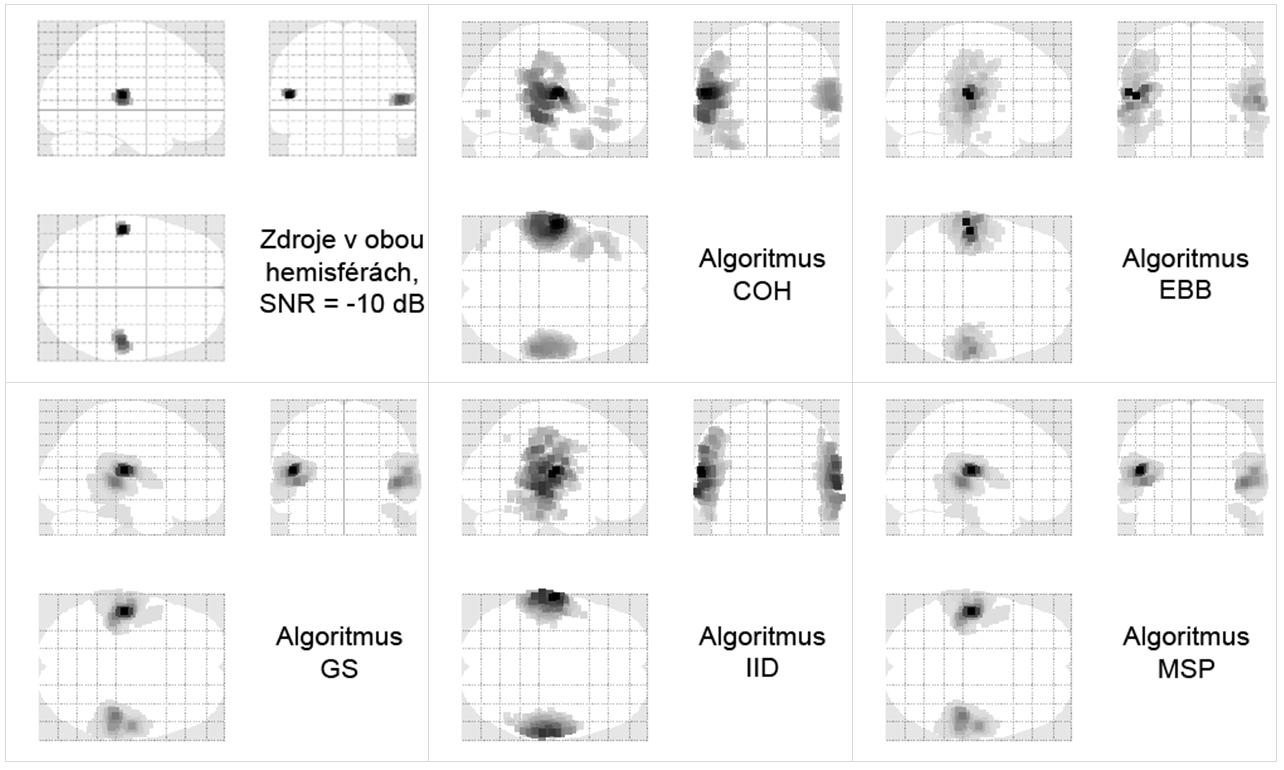
\includegraphics[width=1.0\textwidth]{casti/aplikace/porovnani/scenar5.png}
\caption{Výsledky lokalizace zdroje v pravé i levé hemisféře, při SNR -10 dB}
\label{scenar5}
\end{figure}

\end{itemize}


\subsection{Shrnutí výsledků}
Z těchto scénářů jsem vypočetl průměrné lokalizační chyby jednotlivých algoritmů. Jsou rozepsány v tabulce \ref{prumerneChyby}.

\begin{table}
\begin{ctucolortab}
\begin{tabular}{lp{1.2cm}p{1.2cm}p{1.2cm}p{1.2cm}p{1.2cm}}
\bfseries Algoritmus & COH	& EBB	& GS	& IID	& MSP \\
\Midrule
\bfseries Chyba lokalizace [mm] & 12,7	& 3,7	& 7,8	& 15,5	& 8,7
\end{tabular}
\end{ctucolortab}
\caption{Průměrné chyby lokalizace algoritmů inverzních úloh SPM12 toolboxu}
\label{prumerneChyby}
\end{table}

Z výsledků je možné vyvodit několik závěrů. Metody COH a IID mají tendenci promítat zdroj aktivity k povrchu mozku. U metody IID jsem tuto vlastnost očekával (viz teorie, \ref{minimumNorm}), u metody COH měla však být tato vlastnost kompenzována vhodným váhováním. Algoritmy GS a MSP dávají velmi podobné výsledky, i když MSP je oproti GS výpočetně mnohem náročnější (výpočet GS trvá desítky sekund, výpočet MSP zabere několik hodin). Všechny metody jsou robustní a dávají správné výsledky i v případě, že jsou jednotlivé události velmi zarušené. Důležitou roli zde hraje proces průměrování, ve výsledném signálu je šum dobře potlačen. Výsledky algoritmu EBB jsou velmi fokální, když jsou data generována ze dvou zdrojů, EBB bezpečně najde jeden z nich, druhý potlačí. Tento algoritmus je zároveň nejcitlivější na rušení.


\section{Aplikace inverzních úloh na reálná data}
Pro ověření použitelnosti SPM Motol toolboxu v praxi jsem naimplementované funkce použil při zpracovávání několika případů pacientů. Na případech jsem spolupracoval s pracovníky nemocnice Motol, kteří EEG data naměřili, a s konzultantem Ing. Petrem Ježdíkem, Ph.D.  Převážně se jedná o~zpracování somatosenzorických evokovaných potenciálů, které byly měřeny na epileptických pacientech během několikahodinového snímání. Zpracoval jsem ale i případ epilepsie pacienta.

\subsection{Měření reálných dat}
Měření high density EEG dat v nemocnici Motol provádí MUDr. Adam Kalina a proces měření probíhá následovně. Epileptický pacient se ráno dostaví do nemocnice, kde mu je nasazena čepice, která určuje rozložení elektrod. Za pomoci zdravotní sestry jsou elektrody nagelovány tak, aby byl zajištěn kontakt elektrody a skalpu hlavy, ale zároveň tak, aby nedošlo ke vzniku solných můstků. Následuje snímání pozic elektrod kamerovým systémem. Pacient je 2 hodiny monitorován v bdělém stavu, v tomto období probíhá kognitivní testování. Následují další 2 hodiny monitorace pacienta v leže, pokud možno ve spánku, kdy měření nebývá zatíženo svalovými artefakty. Poslední fází je měření somatozensorických evokovaných potenciálů. Pacient je přesunut do křesla, je mu podložena ruka dekou a MUDr. Kalina začne hledáním nervus medianus pomocí krátkých proudových stimulů. Hledání probíhá na spodní straně zápěstí polohováním dvou elektrod a pozorováním odezvy pacientovy ruky (očekávají se záškuby palce). Upravována je také amplituda stimulů tak, aby záškuby palce byly dostatečně silné a zároveň aby vyšetření nebylo pro pacienta bolestivé. Po nalezení potřebné polohy elektrod a amplitudy stimulů probíhá měření 512 somatosenzorických evokovaných potenciálů se stimulační frekvencí 2 Hz. Proces měření je proveden nejdříve na levé a poté na pravé ruce. Po dokončení této procedury je pacient propuštěn domů. \cite{67}

I když jsou pacienti instruováni, aby se snažili zůstat v klidu a uvolnili svalstvo, aby v záznamu nevznikaly zbytečné artefakty, často se tak neděje. Pacienti se po chvíli začínají nudit a převalují se na posteli. Pro vyhodnocování ložiska epilepsie jsou proto nejvhodnější data, naměřená při spánku, kdy je pacient uvolněný. Podobný problém provází i měření evokovaných potenciálů. Měření je zajímavé, pacient jej sleduje, přičemž se předkloní, aby dobře viděl, tím ale způsobí tonus krčních svalů a svalové artefakty v záznamu. Pokud se svalové artefakty z oblasti krku vyskytují po celou dobu měření somatosenzorických evokovaných potenciálů, průměrování se může stát méně účinným, protože se již nejedná o náhodnou aktivitu.

Pro měření EEG dat je využíván systém Asa-lab, skládající se ze dvou 128 kanálových zesilovačů a čepice s digitizérem od společnosti ANT Neuro. \cite{67}

\subsection{Lokalizace zdroje SEP}
Ideou stojící za prováděním somatosenzorických evokovaných potenciálů během zkoumání ložiska epilepsie je, že umožňují otestovat výsledky inverzní úlohy u konkrétního pacienta, protože u evokovaných potenciálů známe místo a čas, kde se má mozková aktiva objevit.

\subsubsection{Výsledky}
Výsledky byly vypočteny algoritmem LORETA (COH) ve frekvenčním pásmu 1 až 150~Hz, data byla převzorkována na frekvenci 1024 Hz. Využil jsem algoritmu LORETA, protože se v článcích, porovnávajících různé algoritmy umisťoval na prvních příčkách. Vlastní porovnání jsem prováděl až po evaluaci somatosenzorických evokovaných potenciálů.


\paragraph{Pacient P99}
U tohoto pacienta jsou k dispozici pouze data somatosenzorických evokovaných potenciálů levé ruky. Při stimulaci pravé ruky byl vyvolán záchvat (kvůli epileptickému ložisku blízko gyrus postcentralis levé hemisféry) a měření bylo přerušeno.

Ve výsledcích dostupných evokovaných potenciálů je hlavním zdrojem aktivity gyrus postcentralis, objevují se také dlouhodobě přetrvávající ložiska v okcipitální a frontální oblasti, která jsou pravděpodobně způsobena artefakty krčních a očních svalů. Další, méně výrazná, ložiska aktivity, která se objevují blízko primární senzitivní oblasti směrem k frontálnímu laloku, by mohla být způsobena primární a sekundární motorickou oblastí.
\begin{figure}[!h]
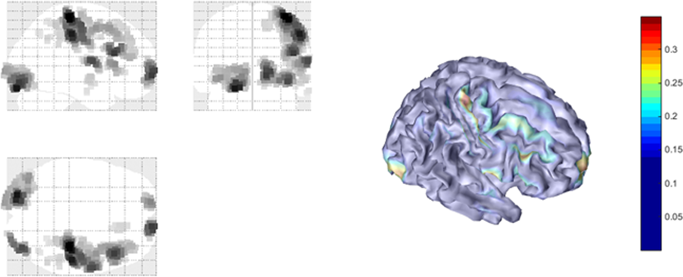
\includegraphics[width=1.0\textwidth]{casti/aplikace/sep/P99.png}
\caption{Výsledek inverzní úlohy evokovaných potenciálů pacienta P99}
\end{figure}

\paragraph{Pacient P109}
Hlavním zdrojem aktivity je primární senzitivní oblast pro ruku, kde aktivitu očekáváme. Ostatní zdroje aktivity jsou jen velmi slabými ložisky, kterým bych nepřikládal význam, protože jde pravděpodobně o náhodnou mozkovou aktivitu.

\begin{figure}[!h]
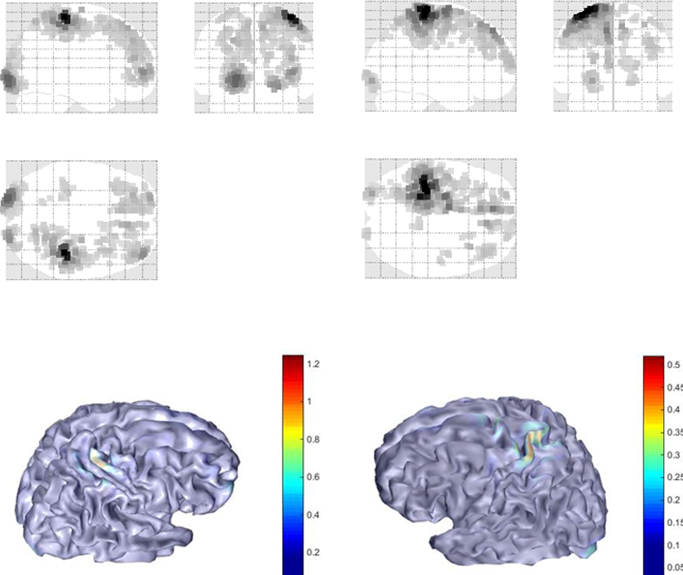
\includegraphics[width=1.0\textwidth]{casti/aplikace/sep/P109.png}
\caption{Výsledek inverzní úlohy evokovaných potenciálů pacienta P109}
\end{figure}

\paragraph{Pacient P110}
Ložiska aktivity jsou v tomto případě opět na očekávaném místě, ostatní zdroje jsou zanedbatelné.

\begin{figure}[!h]
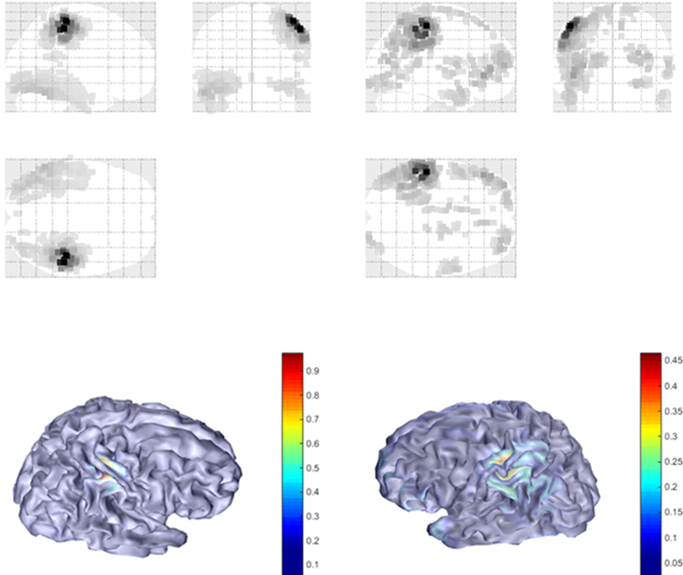
\includegraphics[width=1.0\textwidth]{casti/aplikace/sep/P110.png}
\caption{Výsledek inverzní úlohy evokovaných potenciálů pacienta P110}
\end{figure}

\paragraph{Pacient P113}
V tomto případě, u somatosenzorických evokovaných potenciálů pravé ruky, se opět objevuje silný dlouhodobý zdroj aktivity v okcipitální oblasti, opět asi způsoben svalovým tonem. Můžeme také pozorovat dvě ložiska v obou hemisférách ve frontální laloku. Pravděpodobně jde o jedno ložisko, které je chybně interpretováno inverzní úlohou. Toto ložisko se objevuje během stejného časového intervalu jako aktivita v gyrus postcentralis.
V~případě levé ruky se neobjevuje nic neočekávaného.
Výsledky jsou vykresleny v~obrázku \ref{sepP113}.


\paragraph{Pacient P114}
V případě evokovaných potenciálů levé ruky se aktivita v~primární senzitivní oblasti nečekaně neobjevuje. Objevuje se v primární a~sekundární motorické oblasti, zasahuje však až do spánkového laloku. Bohužel nejsem schopen odůvodnit, proč k tomuto jevu došlo.
V případě měření prováděných za stimulace pravé ruky se již ložisko v gyrus postcentralis pro ruku objevuje, je ale zastíněno vyšší aktivitou gyrus postcentralis pro oblast obličeje.
Výsledky jsou vykresleny v obrázku \ref{sepP114}.

\paragraph{Shrnutí výsledků}
Ve výsledcích somatosenzorických evokovaných potenciálů u všech pacientů (vyjma pacienta P114 evokované potenciály levé ruky) je vidět aktivita na očekávaném místě v gyrus postcentralis.

V některých případech je vidět také aktivita v okcipitální oblasti a frontálním laloku, která přetrvává během celého časového okna. Je pravděpodobně způsobena artefakty krčních a očních svalů.

Občasně je také vidět ložisko aktivity, které nelze vysvětlit svalovými artefakty ani evokovanými potenciály. Taková ložiska ale přetrvávají jen několik časových vzorků, proto si myslím, že jde o náhodnou mozkovou aktivitu, kterou se nepodařilo odstranit průměrováním.

V případě evokovaných potenciálů levé ruky pacienta P114 vidíme výsledek mimo očekávanou oblast, aktivita se objevila o několik centimetrů posunutá směrem k čelnímu laloku. 



\begin{figure}[!p]
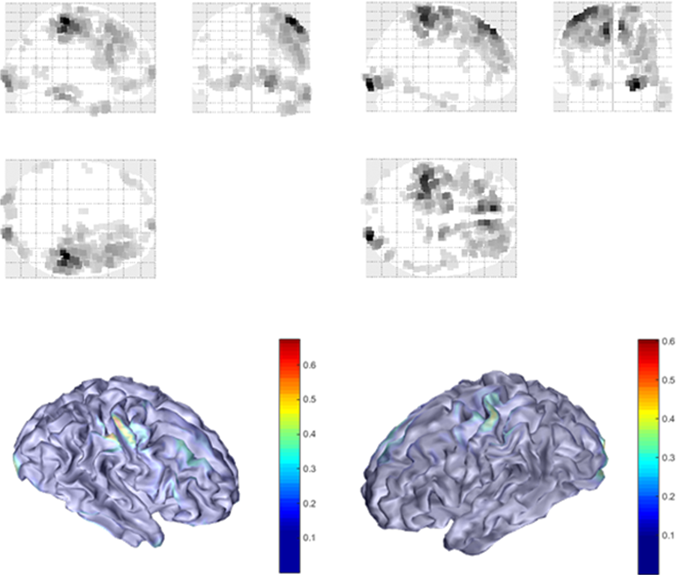
\includegraphics[width=0.9\textwidth]{casti/aplikace/sep/P113.png}
\caption{Výsledek inverzní úlohy evokovaných potenciálů pacienta P113}
\label{sepP113}
\end{figure}

\begin{figure}[!p]
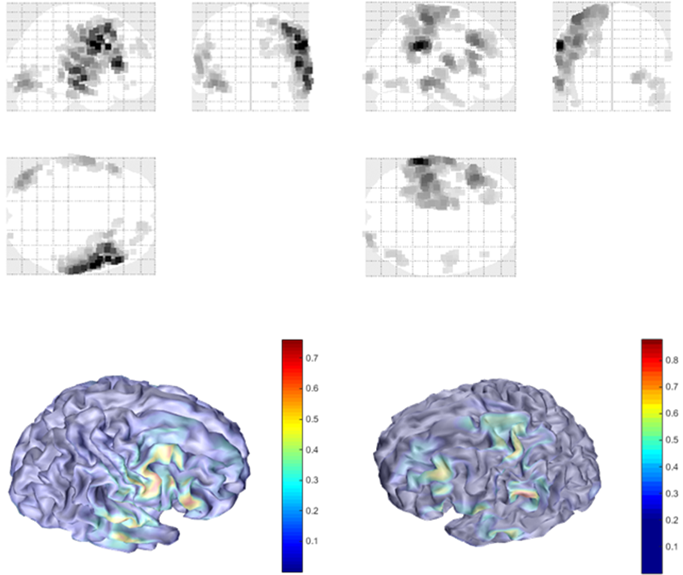
\includegraphics[width=0.9\textwidth]{casti/aplikace/sep/P114.png}
\caption{Výsledek inverzní úlohy evokovaných potenciálů pacienta P114}
\label{sepP114}
\end{figure}




\newpage
\subsection{Lokalizace zdroje epileptické aktivity pacienta P81}

\subsubsection{Tvorba dat}
Data pro analýzu epileptických grafoelementů hrot-vlna a výpočet inverzní úlohy připravil Ing. Petr Ježdík, Ph.D. Ze 110 minut high density záznamu o 256 elektrodách vybral celkem 45 minut záznamu ve spánku, které byly vhodné pro aplikaci automatické detekce komplexů hrot-vlna. Ostatní data obsahovala četné artefakty.

Na vybraná data epileptického pacienta byl aplikován jednokanálový detektor komplexů hrot-vlna, navržený Ing. Radkem Jančou, Ph.D. v článku \cite{70}. Nalezené grafoelementy jsou následně roztříděny do skupin (clusterů) pomocí PCA (Principal Component Analysis) algoritmu. Získané skupiny podobných průběhů jsou následně podrobeny průměrování, získáme tak 1,5 sekundy dlouhý vzorek EEG záznamu příslušného clusteru o 256 kanálech. Jednotlivé průběhy jsou podrobeny vizuální inspekci a jsou vybrány clustery, které skutečně obsahují komplexy hrot-vlna spojené s epilepsií (jiné skupiny mohou obsahovat falešné detekce, jde například o průměty EKG do kanálů EEG, o kterých víme, že jsou také detekovány detektorem; takový cluster je z analýzy vyřazen). Podrobnosti o procesu vytváření clusterů grafoelementů pomocí PCA budou zveřejněny v následujícím článku Ing. Radka Janči, Ph.D. \cite{75}

Nejvíce informací o ložisku epilepsie obsahuje hrot, vlna je pouze následnou odezvou. Hrot se v tomto případě nachází v čase 490 milisekund.
\begin{figure}[!h]
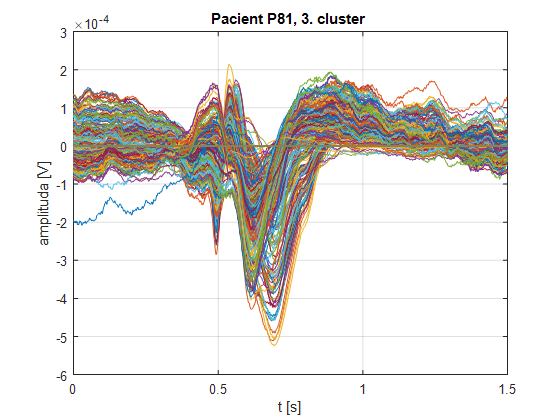
\includegraphics[width=1.0\textwidth]{casti/aplikace/epilepsie/prubehy.png}
\caption{Průměr z komplexů hrot-vlna pacienta P81}
\end{figure}

Ing. Petr Ježdík, Ph.D. také připravil analýzu nad prostorem elektrod, která je znázorněna na obrázku \ref{analyzaElektrod}. Skládá se z grafického vynesení četnosti detekovaných komplexů hrot-vlna za minutu (vyneseno v prvním sloupci), z~pozorovaných amplitud jednotlivých výbojů (druhý sloupec) a ze zobrazení času šíření vzruchu po detekovaném hrotu (sloupec vpravo). Jako vhodné pro aplikaci inverzní úlohy byly vybrány první dva clustery (první cluster v~prvním řádku obrázku \ref{analyzaElektrod}, druhý v druhém), které byly výstupem PCA.
\begin{figure}[!h]
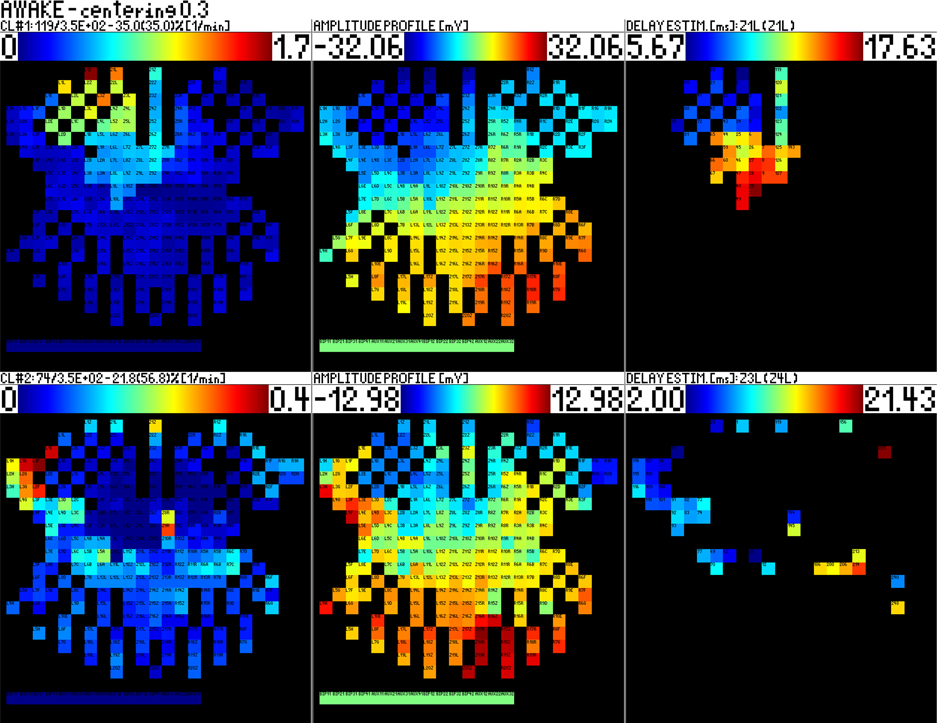
\includegraphics[width=1.0\textwidth]{casti/aplikace/epilepsie/analyza.png}
\caption{Analýza prostoru elektrod}
\label{analyzaElektrod}
\end{figure}

Z této analýzy jsme usoudili, že se očekávané ložisko epileptických výbojů nachází ve frontálním laloku levé hemisféry. V tomto místě bylo detekováno nejvíce komplexů hrot-vlna a odtud se výboj šířil dál do mozku. Výsledek lokalizace prvního clusteru jsem očekával v čelní části levé hemisféry. Ložisko, podle druhého clusteru, by se mělo nacházet v levé hemisféře, několik centimetrů pod Brocovým centrem řeči.
 
Parametry inverze jsem nastavil tak, aby bylo bráno v potaz frekvenční pásmo 16 až 128 Hz. To mi umožní zachovat vysoké frekvence komplexu hrot-vlna a zároveň potlačit pomalé průběhy s vysokou energií, které se mohou jevit jako hlavní ložiska aktivity, i když nemají s epilepsií nic společného. Pro inverzi jsem využil algoritmu LORETA (v SPM12 toolboxu pod zkratkou COH).

\newpage
\subsubsection{Výsledky}

\paragraph{1. cluster}
Na výsledných obrázcích je vidět vykreslení do skleněného mozku (vlevo nahoře), kde jsem označil strany mozku, aby nedošlo k nedorozumění. V pravé horní části je vidět průběh odhadnutý virtuální elektrodou v místě nejvyšší aktivity. Spodní obrázky vykreslují výsledky do trojrozměrného modelu pacientova mozku a do MRI snímků.

\begin{figure}[!h]
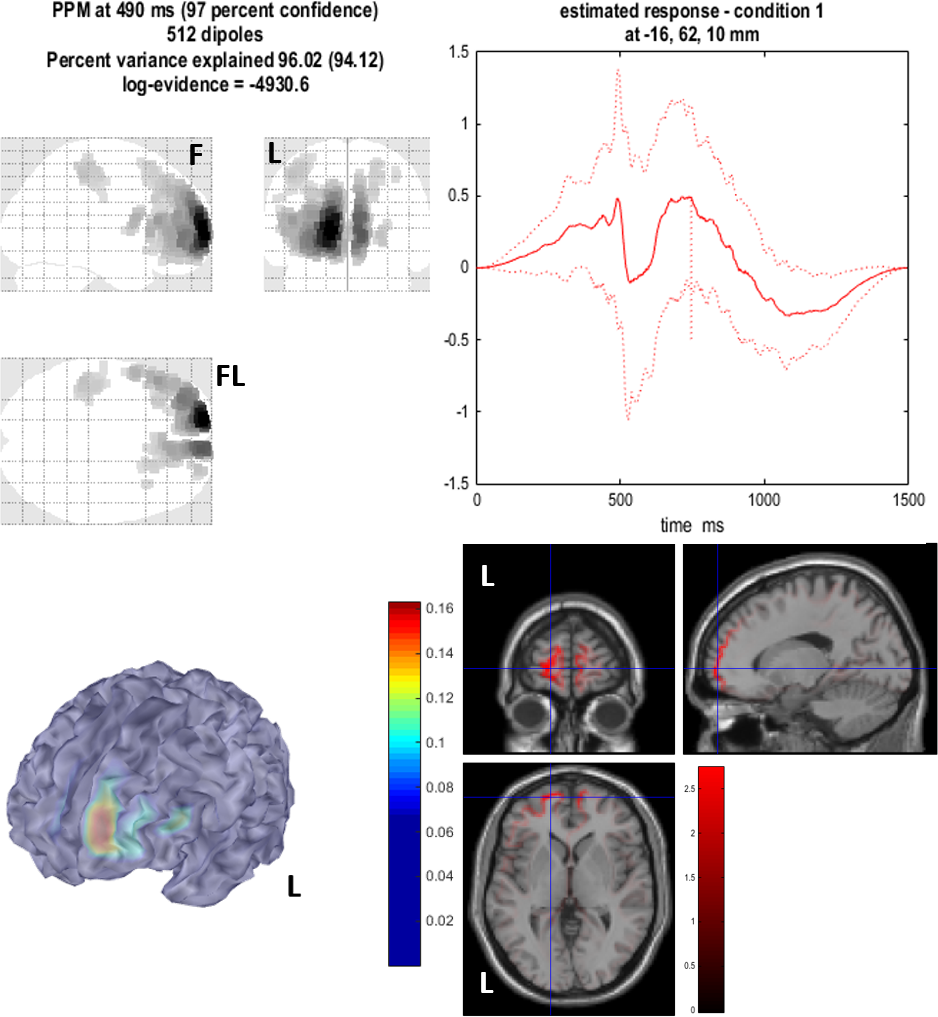
\includegraphics[width=1.0\textwidth]{casti/aplikace/epilepsie/1cl.png}
\caption{Výsledek inverzní úlohy epileptického pacienta P81, 1. cluster}
\end{figure}


\paragraph{2. cluster}
Aktivita tohoto clusteru se objevuje na předpokládaném místě pod Brocovým centrem řeči. Výsledky jsou zobrazeny v obrázku \ref{epilepsieCluster2}.

\begin{figure}[!h]
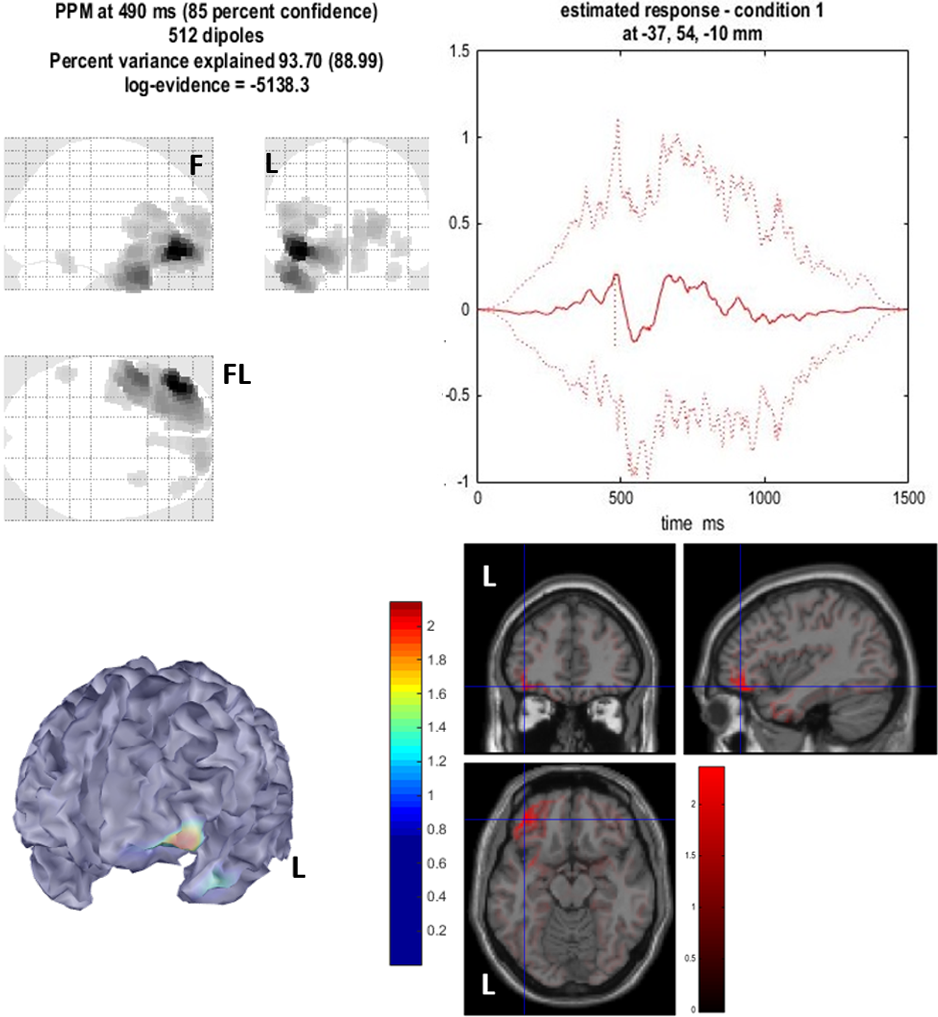
\includegraphics[width=1.0\textwidth]{casti/aplikace/epilepsie/2cl.png}
\caption{Výsledek inverzní úlohy epileptického pacienta P81, 2. cluster}
\label{epilepsieCluster2}
\end{figure}

\paragraph{3. cluster}
Tento cluster, také vhodný pro aplikaci inverzní úlohy, byl nalezen při dalším zpracování algoritmem PCA. Očekávám podobný výsledek jako u~prvního clusteru. Výsledky jsou zobrazeny v obrázku \ref{epilepsieCluster3}.

\begin{figure}[!h]
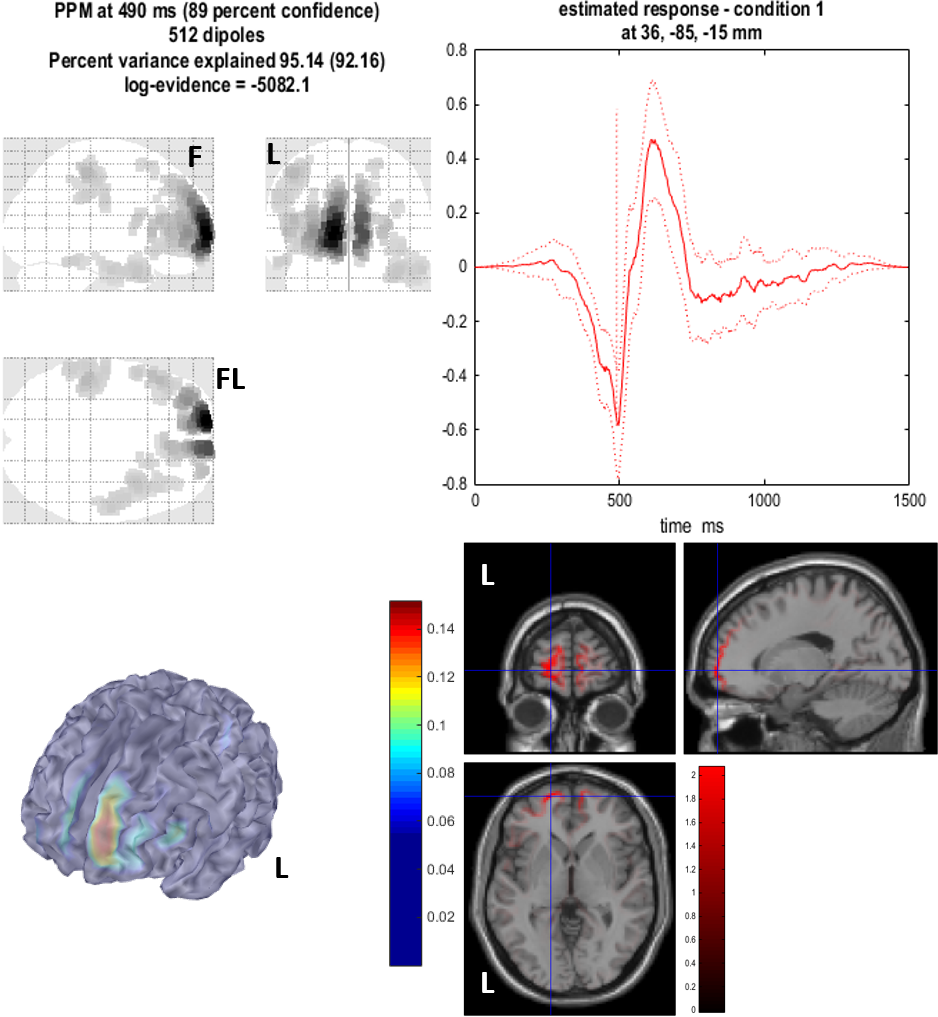
\includegraphics[width=1.0\textwidth]{casti/aplikace/epilepsie/3cl.png}
\caption{Výsledek inverzní úlohy epileptického pacienta P81, 3. cluster}
\label{epilepsieCluster3}
\end{figure}

\paragraph{Shrnutí}
Výsledek inverze potvrzuje očekávání předchozí analýzy. Hlavní ložisko aktivity se nachází ve frontálním laloku levé hemisféry. Ložisko je nejlépe zřetelné v čase 490 ms, tedy v čase, kde se nachází hrot komplexu hrot-vlna. Výsledné ložisko vypadá, jako by zasahovalo také do druhé hemisféry, ve skutečnosti tomu tak není, inverzní metody neumí rozlišovat mezi funkčně odlišnými celky, jako jsou například hemisféry. Takové chyby je možné vyloučit vhodnou interpretací výsledků. 